% Created by tikzDevice version 0.12 on 2019-03-27 17:35:03
% !TEX encoding = UTF-8 Unicode
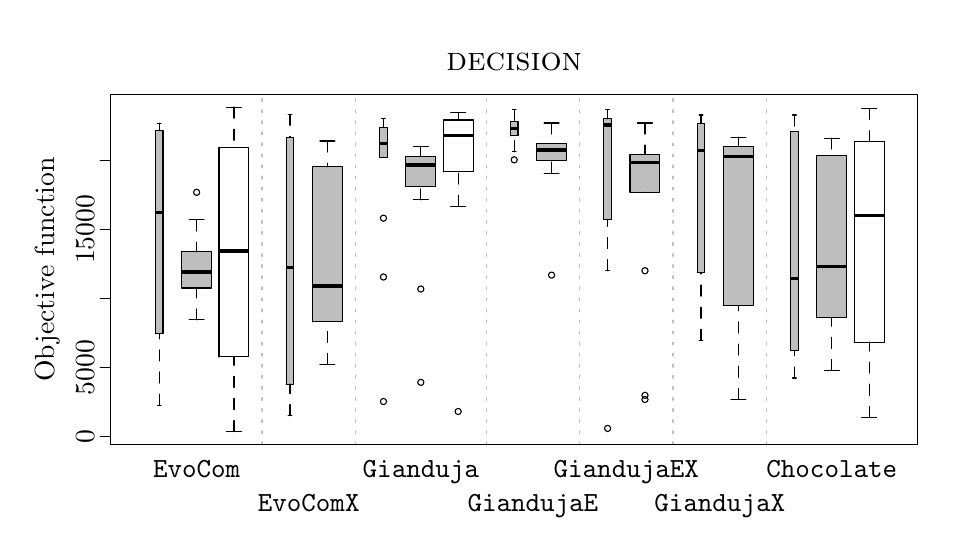
\begin{tikzpicture}[x=1pt,y=1pt]
\definecolor{fillColor}{RGB}{255,255,255}
\path[use as bounding box,fill=fillColor,fill opacity=0.00] (0,0) rectangle (325.21,180.67);
\begin{scope}
\path[clip] ( 30.00, 30.00) rectangle (321.61,156.67);
\definecolor{fillColor}{RGB}{190,190,190}

\path[fill=fillColor] ( 46.20, 70.05) --
	( 48.90, 70.05) --
	( 48.90,143.45) --
	( 46.20,143.45) --
	cycle;
\definecolor{drawColor}{RGB}{0,0,0}

\path[draw=drawColor,line width= 1.2pt,line join=round] ( 46.20,113.98) -- ( 48.90,113.98);

\path[draw=drawColor,line width= 0.4pt,dash pattern=on 4pt off 4pt ,line join=round,line cap=round] ( 47.55, 44.24) -- ( 47.55, 70.05);

\path[draw=drawColor,line width= 0.4pt,dash pattern=on 4pt off 4pt ,line join=round,line cap=round] ( 47.55,146.18) -- ( 47.55,143.45);

\path[draw=drawColor,line width= 0.4pt,line join=round,line cap=round] ( 46.88, 44.24) -- ( 48.23, 44.24);

\path[draw=drawColor,line width= 0.4pt,line join=round,line cap=round] ( 46.88,146.18) -- ( 48.23,146.18);

\path[draw=drawColor,line width= 0.4pt,line join=round,line cap=round] ( 46.20, 70.05) --
	( 48.90, 70.05) --
	( 48.90,143.45) --
	( 46.20,143.45) --
	( 46.20, 70.05);

\path[fill=fillColor] ( 55.65, 86.60) --
	( 66.45, 86.60) --
	( 66.45, 99.67) --
	( 55.65, 99.67) --
	cycle;

\path[draw=drawColor,line width= 1.2pt,line join=round] ( 55.65, 92.41) -- ( 66.45, 92.41);

\path[draw=drawColor,line width= 0.4pt,dash pattern=on 4pt off 4pt ,line join=round,line cap=round] ( 61.05, 75.08) -- ( 61.05, 86.60);

\path[draw=drawColor,line width= 0.4pt,dash pattern=on 4pt off 4pt ,line join=round,line cap=round] ( 61.05,111.20) -- ( 61.05, 99.67);

\path[draw=drawColor,line width= 0.4pt,line join=round,line cap=round] ( 58.35, 75.08) -- ( 63.75, 75.08);

\path[draw=drawColor,line width= 0.4pt,line join=round,line cap=round] ( 58.35,111.20) -- ( 63.75,111.20);

\path[draw=drawColor,line width= 0.4pt,line join=round,line cap=round] ( 55.65, 86.60) --
	( 66.45, 86.60) --
	( 66.45, 99.67) --
	( 55.65, 99.67) --
	( 55.65, 86.60);

\path[draw=drawColor,line width= 0.4pt,line join=round,line cap=round] ( 61.05,121.18) circle (  1.12);
\definecolor{fillColor}{RGB}{255,255,255}

\path[fill=fillColor] ( 69.15, 61.71) --
	( 79.95, 61.71) --
	( 79.95,137.32) --
	( 69.15,137.32) --
	cycle;

\path[draw=drawColor,line width= 1.2pt,line join=round] ( 69.15, 99.93) -- ( 79.95, 99.93);

\path[draw=drawColor,line width= 0.4pt,dash pattern=on 4pt off 4pt ,line join=round,line cap=round] ( 74.55, 34.69) -- ( 74.55, 61.71);

\path[draw=drawColor,line width= 0.4pt,dash pattern=on 4pt off 4pt ,line join=round,line cap=round] ( 74.55,151.98) -- ( 74.55,137.32);

\path[draw=drawColor,line width= 0.4pt,line join=round,line cap=round] ( 71.85, 34.69) -- ( 77.25, 34.69);

\path[draw=drawColor,line width= 0.4pt,line join=round,line cap=round] ( 71.85,151.98) -- ( 77.25,151.98);

\path[draw=drawColor,line width= 0.4pt,line join=round,line cap=round] ( 69.15, 61.71) --
	( 79.95, 61.71) --
	( 79.95,137.32) --
	( 69.15,137.32) --
	( 69.15, 61.71);
\definecolor{fillColor}{RGB}{190,190,190}

\path[fill=fillColor] ( 93.45, 51.87) --
	( 96.15, 51.87) --
	( 96.15,141.12) --
	( 93.45,141.12) --
	cycle;

\path[draw=drawColor,line width= 1.2pt,line join=round] ( 93.45, 94.06) -- ( 96.15, 94.06);

\path[draw=drawColor,line width= 0.4pt,dash pattern=on 4pt off 4pt ,line join=round,line cap=round] ( 94.80, 40.46) -- ( 94.80, 51.87);

\path[draw=drawColor,line width= 0.4pt,dash pattern=on 4pt off 4pt ,line join=round,line cap=round] ( 94.80,149.38) -- ( 94.80,141.12);

\path[draw=drawColor,line width= 0.4pt,line join=round,line cap=round] ( 94.13, 40.46) -- ( 95.48, 40.46);

\path[draw=drawColor,line width= 0.4pt,line join=round,line cap=round] ( 94.13,149.38) -- ( 95.48,149.38);

\path[draw=drawColor,line width= 0.4pt,line join=round,line cap=round] ( 93.45, 51.87) --
	( 96.15, 51.87) --
	( 96.15,141.12) --
	( 93.45,141.12) --
	( 93.45, 51.87);

\path[fill=fillColor] (102.90, 74.35) --
	(113.70, 74.35) --
	(113.70,130.35) --
	(102.90,130.35) --
	cycle;

\path[draw=drawColor,line width= 1.2pt,line join=round] (102.90, 87.33) -- (113.70, 87.33);

\path[draw=drawColor,line width= 0.4pt,dash pattern=on 4pt off 4pt ,line join=round,line cap=round] (108.30, 58.94) -- (108.30, 74.35);

\path[draw=drawColor,line width= 0.4pt,dash pattern=on 4pt off 4pt ,line join=round,line cap=round] (108.30,139.73) -- (108.30,130.35);

\path[draw=drawColor,line width= 0.4pt,line join=round,line cap=round] (105.60, 58.94) -- (111.00, 58.94);

\path[draw=drawColor,line width= 0.4pt,line join=round,line cap=round] (105.60,139.73) -- (111.00,139.73);

\path[draw=drawColor,line width= 0.4pt,line join=round,line cap=round] (102.90, 74.35) --
	(113.70, 74.35) --
	(113.70,130.35) --
	(102.90,130.35) --
	(102.90, 74.35);

\path[fill=fillColor] (127.20,133.87) --
	(129.91,133.87) --
	(129.91,144.71) --
	(127.20,144.71) --
	cycle;

\path[draw=drawColor,line width= 1.2pt,line join=round] (127.20,138.76) -- (129.91,138.76);

\path[draw=drawColor,line width= 0.4pt,dash pattern=on 4pt off 4pt ,line join=round,line cap=round] (128.56,133.87) -- (128.56,133.87);

\path[draw=drawColor,line width= 0.4pt,dash pattern=on 4pt off 4pt ,line join=round,line cap=round] (128.56,147.74) -- (128.56,144.71);

\path[draw=drawColor,line width= 0.4pt,line join=round,line cap=round] (127.88,133.87) -- (129.23,133.87);

\path[draw=drawColor,line width= 0.4pt,line join=round,line cap=round] (127.88,147.74) -- (129.23,147.74);

\path[draw=drawColor,line width= 0.4pt,line join=round,line cap=round] (127.20,133.87) --
	(129.91,133.87) --
	(129.91,144.71) --
	(127.20,144.71) --
	(127.20,133.87);

\path[draw=drawColor,line width= 0.4pt,line join=round,line cap=round] (128.56, 90.56) circle (  1.12);

\path[draw=drawColor,line width= 0.4pt,line join=round,line cap=round] (128.56, 45.58) circle (  1.12);

\path[draw=drawColor,line width= 0.4pt,line join=round,line cap=round] (128.56,111.83) circle (  1.12);

\path[fill=fillColor] (136.66,123.23) --
	(147.46,123.23) --
	(147.46,134.23) --
	(136.66,134.23) --
	cycle;

\path[draw=drawColor,line width= 1.2pt,line join=round] (136.66,131.08) -- (147.46,131.08);

\path[draw=drawColor,line width= 0.4pt,dash pattern=on 4pt off 4pt ,line join=round,line cap=round] (142.06,118.44) -- (142.06,123.23);

\path[draw=drawColor,line width= 0.4pt,dash pattern=on 4pt off 4pt ,line join=round,line cap=round] (142.06,137.80) -- (142.06,134.23);

\path[draw=drawColor,line width= 0.4pt,line join=round,line cap=round] (139.36,118.44) -- (144.76,118.44);

\path[draw=drawColor,line width= 0.4pt,line join=round,line cap=round] (139.36,137.80) -- (144.76,137.80);

\path[draw=drawColor,line width= 0.4pt,line join=round,line cap=round] (136.66,123.23) --
	(147.46,123.23) --
	(147.46,134.23) --
	(136.66,134.23) --
	(136.66,123.23);

\path[draw=drawColor,line width= 0.4pt,line join=round,line cap=round] (142.06, 86.24) circle (  1.12);

\path[draw=drawColor,line width= 0.4pt,line join=round,line cap=round] (142.06, 52.50) circle (  1.12);
\definecolor{fillColor}{RGB}{255,255,255}

\path[fill=fillColor] (150.16,128.56) --
	(160.96,128.56) --
	(160.96,147.30) --
	(150.16,147.30) --
	cycle;

\path[draw=drawColor,line width= 1.2pt,line join=round] (150.16,141.76) -- (160.96,141.76);

\path[draw=drawColor,line width= 0.4pt,dash pattern=on 4pt off 4pt ,line join=round,line cap=round] (155.56,116.14) -- (155.56,128.56);

\path[draw=drawColor,line width= 0.4pt,dash pattern=on 4pt off 4pt ,line join=round,line cap=round] (155.56,149.89) -- (155.56,147.30);

\path[draw=drawColor,line width= 0.4pt,line join=round,line cap=round] (152.86,116.14) -- (158.26,116.14);

\path[draw=drawColor,line width= 0.4pt,line join=round,line cap=round] (152.86,149.89) -- (158.26,149.89);

\path[draw=drawColor,line width= 0.4pt,line join=round,line cap=round] (150.16,128.56) --
	(160.96,128.56) --
	(160.96,147.30) --
	(150.16,147.30) --
	(150.16,128.56);

\path[draw=drawColor,line width= 0.4pt,line join=round,line cap=round] (155.56, 41.98) circle (  1.12);
\definecolor{fillColor}{RGB}{190,190,190}

\path[fill=fillColor] (174.46,141.60) --
	(177.16,141.60) --
	(177.16,146.74) --
	(174.46,146.74) --
	cycle;

\path[draw=drawColor,line width= 1.2pt,line join=round] (174.46,144.33) -- (177.16,144.33);

\path[draw=drawColor,line width= 0.4pt,dash pattern=on 4pt off 4pt ,line join=round,line cap=round] (175.81,135.84) -- (175.81,141.60);

\path[draw=drawColor,line width= 0.4pt,dash pattern=on 4pt off 4pt ,line join=round,line cap=round] (175.81,151.14) -- (175.81,146.74);

\path[draw=drawColor,line width= 0.4pt,line join=round,line cap=round] (175.13,135.84) -- (176.48,135.84);

\path[draw=drawColor,line width= 0.4pt,line join=round,line cap=round] (175.13,151.14) -- (176.48,151.14);

\path[draw=drawColor,line width= 0.4pt,line join=round,line cap=round] (174.46,141.60) --
	(177.16,141.60) --
	(177.16,146.74) --
	(174.46,146.74) --
	(174.46,141.60);

\path[draw=drawColor,line width= 0.4pt,line join=round,line cap=round] (175.81,132.91) circle (  1.12);

\path[fill=fillColor] (183.91,132.72) --
	(194.71,132.72) --
	(194.71,138.85) --
	(183.91,138.85) --
	cycle;

\path[draw=drawColor,line width= 1.2pt,line join=round] (183.91,136.42) -- (194.71,136.42);

\path[draw=drawColor,line width= 0.4pt,dash pattern=on 4pt off 4pt ,line join=round,line cap=round] (189.31,128.09) -- (189.31,132.72);

\path[draw=drawColor,line width= 0.4pt,dash pattern=on 4pt off 4pt ,line join=round,line cap=round] (189.31,146.23) -- (189.31,138.85);

\path[draw=drawColor,line width= 0.4pt,line join=round,line cap=round] (186.61,128.09) -- (192.01,128.09);

\path[draw=drawColor,line width= 0.4pt,line join=round,line cap=round] (186.61,146.23) -- (192.01,146.23);

\path[draw=drawColor,line width= 0.4pt,line join=round,line cap=round] (183.91,132.72) --
	(194.71,132.72) --
	(194.71,138.85) --
	(183.91,138.85) --
	(183.91,132.72);

\path[draw=drawColor,line width= 0.4pt,line join=round,line cap=round] (189.31, 91.25) circle (  1.12);

\path[fill=fillColor] (208.21,111.42) --
	(210.91,111.42) --
	(210.91,147.74) --
	(208.21,147.74) --
	cycle;

\path[draw=drawColor,line width= 1.2pt,line join=round] (208.21,145.50) -- (210.91,145.50);

\path[draw=drawColor,line width= 0.4pt,dash pattern=on 4pt off 4pt ,line join=round,line cap=round] (209.56, 92.84) -- (209.56,111.42);

\path[draw=drawColor,line width= 0.4pt,dash pattern=on 4pt off 4pt ,line join=round,line cap=round] (209.56,151.14) -- (209.56,147.74);

\path[draw=drawColor,line width= 0.4pt,line join=round,line cap=round] (208.88, 92.84) -- (210.23, 92.84);

\path[draw=drawColor,line width= 0.4pt,line join=round,line cap=round] (208.88,151.14) -- (210.23,151.14);

\path[draw=drawColor,line width= 0.4pt,line join=round,line cap=round] (208.21,111.42) --
	(210.91,111.42) --
	(210.91,147.74) --
	(208.21,147.74) --
	(208.21,111.42);

\path[draw=drawColor,line width= 0.4pt,line join=round,line cap=round] (209.56, 35.86) circle (  1.12);

\path[fill=fillColor] (217.66,121.22) --
	(228.46,121.22) --
	(228.46,134.81) --
	(217.66,134.81) --
	cycle;

\path[draw=drawColor,line width= 1.2pt,line join=round] (217.66,131.96) -- (228.46,131.96);

\path[draw=drawColor,line width= 0.4pt,dash pattern=on 4pt off 4pt ,line join=round,line cap=round] (223.06,121.22) -- (223.06,121.22);

\path[draw=drawColor,line width= 0.4pt,dash pattern=on 4pt off 4pt ,line join=round,line cap=round] (223.06,146.23) -- (223.06,134.81);

\path[draw=drawColor,line width= 0.4pt,line join=round,line cap=round] (220.36,121.22) -- (225.76,121.22);

\path[draw=drawColor,line width= 0.4pt,line join=round,line cap=round] (220.36,146.23) -- (225.76,146.23);

\path[draw=drawColor,line width= 0.4pt,line join=round,line cap=round] (217.66,121.22) --
	(228.46,121.22) --
	(228.46,134.81) --
	(217.66,134.81) --
	(217.66,121.22);

\path[draw=drawColor,line width= 0.4pt,line join=round,line cap=round] (223.06, 92.84) circle (  1.12);

\path[draw=drawColor,line width= 0.4pt,line join=round,line cap=round] (223.06, 46.32) circle (  1.12);

\path[draw=drawColor,line width= 0.4pt,line join=round,line cap=round] (223.06, 47.81) circle (  1.12);

\path[fill=fillColor] (241.96, 92.16) --
	(244.66, 92.16) --
	(244.66,146.12) --
	(241.96,146.12) --
	cycle;

\path[draw=drawColor,line width= 1.2pt,line join=round] (241.96,136.24) -- (244.66,136.24);

\path[draw=drawColor,line width= 0.4pt,dash pattern=on 4pt off 4pt ,line join=round,line cap=round] (243.31, 67.67) -- (243.31, 92.16);

\path[draw=drawColor,line width= 0.4pt,dash pattern=on 4pt off 4pt ,line join=round,line cap=round] (243.31,149.13) -- (243.31,146.12);

\path[draw=drawColor,line width= 0.4pt,line join=round,line cap=round] (242.64, 67.67) -- (243.99, 67.67);

\path[draw=drawColor,line width= 0.4pt,line join=round,line cap=round] (242.64,149.13) -- (243.99,149.13);

\path[draw=drawColor,line width= 0.4pt,line join=round,line cap=round] (241.96, 92.16) --
	(244.66, 92.16) --
	(244.66,146.12) --
	(241.96,146.12) --
	(241.96, 92.16);

\path[fill=fillColor] (251.41, 80.22) --
	(262.21, 80.22) --
	(262.21,137.78) --
	(251.41,137.78) --
	cycle;

\path[draw=drawColor,line width= 1.2pt,line join=round] (251.41,134.12) -- (262.21,134.12);

\path[draw=drawColor,line width= 0.4pt,dash pattern=on 4pt off 4pt ,line join=round,line cap=round] (256.81, 46.32) -- (256.81, 80.22);

\path[draw=drawColor,line width= 0.4pt,dash pattern=on 4pt off 4pt ,line join=round,line cap=round] (256.81,141.13) -- (256.81,137.78);

\path[draw=drawColor,line width= 0.4pt,line join=round,line cap=round] (254.11, 46.32) -- (259.51, 46.32);

\path[draw=drawColor,line width= 0.4pt,line join=round,line cap=round] (254.11,141.13) -- (259.51,141.13);

\path[draw=drawColor,line width= 0.4pt,line join=round,line cap=round] (251.41, 80.22) --
	(262.21, 80.22) --
	(262.21,137.78) --
	(251.41,137.78) --
	(251.41, 80.22);

\path[fill=fillColor] (275.71, 64.00) --
	(278.41, 64.00) --
	(278.41,143.20) --
	(275.71,143.20) --
	cycle;

\path[draw=drawColor,line width= 1.2pt,line join=round] (275.71, 90.01) -- (278.41, 90.01);

\path[draw=drawColor,line width= 0.4pt,dash pattern=on 4pt off 4pt ,line join=round,line cap=round] (277.06, 54.08) -- (277.06, 64.00);

\path[draw=drawColor,line width= 0.4pt,dash pattern=on 4pt off 4pt ,line join=round,line cap=round] (277.06,149.13) -- (277.06,143.20);

\path[draw=drawColor,line width= 0.4pt,line join=round,line cap=round] (276.39, 54.08) -- (277.74, 54.08);

\path[draw=drawColor,line width= 0.4pt,line join=round,line cap=round] (276.39,149.13) -- (277.74,149.13);

\path[draw=drawColor,line width= 0.4pt,line join=round,line cap=round] (275.71, 64.00) --
	(278.41, 64.00) --
	(278.41,143.20) --
	(275.71,143.20) --
	(275.71, 64.00);

\path[fill=fillColor] (285.16, 75.79) --
	(295.96, 75.79) --
	(295.96,134.63) --
	(285.16,134.63) --
	cycle;

\path[draw=drawColor,line width= 1.2pt,line join=round] (285.16, 94.49) -- (295.96, 94.49);

\path[draw=drawColor,line width= 0.4pt,dash pattern=on 4pt off 4pt ,line join=round,line cap=round] (290.56, 56.79) -- (290.56, 75.79);

\path[draw=drawColor,line width= 0.4pt,dash pattern=on 4pt off 4pt ,line join=round,line cap=round] (290.56,140.78) -- (290.56,134.63);

\path[draw=drawColor,line width= 0.4pt,line join=round,line cap=round] (287.86, 56.79) -- (293.26, 56.79);

\path[draw=drawColor,line width= 0.4pt,line join=round,line cap=round] (287.86,140.78) -- (293.26,140.78);

\path[draw=drawColor,line width= 0.4pt,line join=round,line cap=round] (285.16, 75.79) --
	(295.96, 75.79) --
	(295.96,134.63) --
	(285.16,134.63) --
	(285.16, 75.79);
\definecolor{fillColor}{RGB}{255,255,255}

\path[fill=fillColor] (298.66, 66.99) --
	(309.46, 66.99) --
	(309.46,139.48) --
	(298.66,139.48) --
	cycle;

\path[draw=drawColor,line width= 1.2pt,line join=round] (298.66,112.85) -- (309.46,112.85);

\path[draw=drawColor,line width= 0.4pt,dash pattern=on 4pt off 4pt ,line join=round,line cap=round] (304.06, 39.82) -- (304.06, 66.99);

\path[draw=drawColor,line width= 0.4pt,dash pattern=on 4pt off 4pt ,line join=round,line cap=round] (304.06,151.50) -- (304.06,139.48);

\path[draw=drawColor,line width= 0.4pt,line join=round,line cap=round] (301.36, 39.82) -- (306.76, 39.82);

\path[draw=drawColor,line width= 0.4pt,line join=round,line cap=round] (301.36,151.50) -- (306.76,151.50);

\path[draw=drawColor,line width= 0.4pt,line join=round,line cap=round] (298.66, 66.99) --
	(309.46, 66.99) --
	(309.46,139.48) --
	(298.66,139.48) --
	(298.66, 66.99);
\definecolor{drawColor}{RGB}{190,190,190}

\path[draw=drawColor,line width= 0.4pt,dash pattern=on 1pt off 3pt ,line join=round,line cap=round] ( 84.68, 30.00) -- ( 84.68,156.67);

\path[draw=drawColor,line width= 0.4pt,dash pattern=on 1pt off 3pt ,line join=round,line cap=round] (118.43, 30.00) -- (118.43,156.67);

\path[draw=drawColor,line width= 0.4pt,dash pattern=on 1pt off 3pt ,line join=round,line cap=round] (165.68, 30.00) -- (165.68,156.67);

\path[draw=drawColor,line width= 0.4pt,dash pattern=on 1pt off 3pt ,line join=round,line cap=round] (199.43, 30.00) -- (199.43,156.67);

\path[draw=drawColor,line width= 0.4pt,dash pattern=on 1pt off 3pt ,line join=round,line cap=round] (233.19, 30.00) -- (233.19,156.67);

\path[draw=drawColor,line width= 0.4pt,dash pattern=on 1pt off 3pt ,line join=round,line cap=round] (266.94, 30.00) -- (266.94,156.67);
\end{scope}
\begin{scope}
\path[clip] (  0.00,  0.00) rectangle (325.21,180.67);
\definecolor{drawColor}{RGB}{0,0,0}

\node[text=drawColor,anchor=base,inner sep=0pt, outer sep=0pt, scale=  1.00] at ( 61.05, 18.00) {\texttt{EvoCom}};

\node[text=drawColor,anchor=base,inner sep=0pt, outer sep=0pt, scale=  1.00] at (142.06, 18.00) {\texttt{Gianduja}};

\node[text=drawColor,anchor=base,inner sep=0pt, outer sep=0pt, scale=  1.00] at (216.31, 18.00) {\texttt{GiandujaEX}};

\node[text=drawColor,anchor=base,inner sep=0pt, outer sep=0pt, scale=  1.00] at (290.56, 18.00) {\texttt{Chocolate}};

\node[text=drawColor,anchor=base,inner sep=0pt, outer sep=0pt, scale=  1.00] at (101.55,  6.00) {\texttt{EvoComX}};

\node[text=drawColor,anchor=base,inner sep=0pt, outer sep=0pt, scale=  1.00] at (182.56,  6.00) {\texttt{GiandujaE}};

\node[text=drawColor,anchor=base,inner sep=0pt, outer sep=0pt, scale=  1.00] at (250.06,  6.00) {\texttt{GiandujaX}};
\end{scope}
\begin{scope}
\path[clip] (  0.00,  0.00) rectangle (325.21,180.67);
\definecolor{drawColor}{RGB}{0,0,0}

\node[text=drawColor,anchor=base,inner sep=0pt, outer sep=0pt, scale=  1.20] at (175.81,165.07) {\textsc{decision}};

\node[text=drawColor,rotate= 90.00,anchor=base,inner sep=0pt, outer sep=0pt, scale=  1.00] at (  9.60, 93.34) {Objective function};
\end{scope}
\begin{scope}
\path[clip] (  0.00,  0.00) rectangle (325.21,180.67);
\definecolor{drawColor}{RGB}{0,0,0}

\path[draw=drawColor,line width= 0.4pt,line join=round,line cap=round] ( 30.00, 32.88) -- ( 30.00,132.81);

\path[draw=drawColor,line width= 0.4pt,line join=round,line cap=round] ( 30.00, 32.88) -- ( 26.20, 32.88);

\path[draw=drawColor,line width= 0.4pt,line join=round,line cap=round] ( 30.00, 57.86) -- ( 26.20, 57.86);

\path[draw=drawColor,line width= 0.4pt,line join=round,line cap=round] ( 30.00, 82.84) -- ( 26.20, 82.84);

\path[draw=drawColor,line width= 0.4pt,line join=round,line cap=round] ( 30.00,107.82) -- ( 26.20,107.82);

\path[draw=drawColor,line width= 0.4pt,line join=round,line cap=round] ( 30.00,132.81) -- ( 26.20,132.81);

\node[text=drawColor,rotate= 90.00,anchor=base,inner sep=0pt, outer sep=0pt, scale=  1.00] at ( 24.00, 32.88) {0};

\node[text=drawColor,rotate= 90.00,anchor=base,inner sep=0pt, outer sep=0pt, scale=  1.00] at ( 24.00, 57.86) {5000};

\node[text=drawColor,rotate= 90.00,anchor=base,inner sep=0pt, outer sep=0pt, scale=  1.00] at ( 24.00,107.82) {15000};

\path[draw=drawColor,line width= 0.4pt,line join=round,line cap=round] ( 30.00, 30.00) --
	(321.61, 30.00) --
	(321.61,156.67) --
	( 30.00,156.67) --
	( 30.00, 30.00);
\end{scope}
\end{tikzpicture}
